%Einleitung.tex
%
\chapter{Introduction}
\section{Testing}
Software testing refers in the IT-Branch to a product with the main goal of finding bugs in a software program or application. These bugs refer to errors or faults and can occur because of a bad commands sequence specified in the program's source code.\\
A successful test can be achieved when its main requirements are met. Some examples would be the execution on different environments, time constraints or delivering expected outputs for randomly chosen inputs. Conditions are set by the tester and may vary depending on the use case.\\
\section{Motivation}
Most companies put a lot of effort in delivering high performance products to their customers. In order to do so, each of them test their gadgets, machines or software for possible failure scenarios. Now-a-days tests are being fully automated, which decreases the failure possibility that can happen because of human errors.\cite{8389562}\\ Unfortunately the creation of fully automated tests is not as easy as it may sound. Many testing developers know the struggle of finding the right tools for the job and by the end of testing phase, their project is filled with unnecessary dependencies that will overload the program and occupy valuable memory.
\begin{center}
	\say{As ironic as it seems, the challenge of a tester is to test as little as possible. Test less, but test smarter}
	\begin{flushright}
		\textit{Federico Teldo, Co-Founder Abstracta US}
	\end{flushright}
\end{center}
Additionally the problem enhances when a company reaches a certain size with a significant number of customers, which tend to run the product on different machines and architectures. In order to keep their customers, producers need to adapt their products to support newer or older machines. This makes software analysis even more difficult because of the increasing complexity, which comes with different systems. For this reason many companies dedicated themselves to creating programs that focus only on software examination and fixing. In time a new trend has been created with demands so high that rapidly developed itself into a new market section.\\
\section{Growing markets}
For the last decade the software testing market has been developing and now it has grown so big that it would be foolish to ignore it. According to \dq Global Market Insights\dq{} the testing software market has grown up to 40 billion dollars by the end of 2020 and is predicted to grow up to 60 billion dollars in the next 6 years.\cite{GMI}\\
\textit{\dq People may lie, but number don't\dq}. Multiple scientific papers and studies enforce this statement with different statistics of industries, which started adapting and reacting to this trend using the model \dq EaaS \dq{} which stands for \dq Everything as a service\dq{} and created \dq Testing as a Service\dq{}(TaaS). With this model customers not only pay for the current state of a product, but also for a service subscription, where they get updates and new features for the specific product and additional support from the company. The advantages that benefit the customer are set by the company for each of their subscription. (The basic rule is that you get more accurate results if you pay more). This service usually targets three groups: Developers, End Users and Certification Services.\cite{10.1145/1807128.1807153} 
\begin{figure}[htbp]
	\centering
	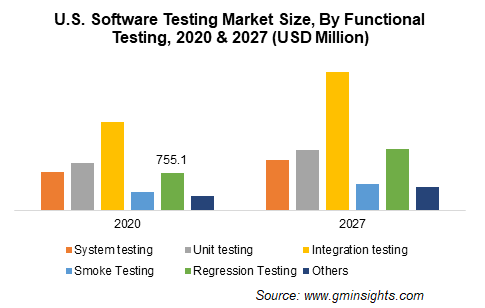
\includegraphics[width=0.80\textwidth]{../figures/einleitung/US_marketsize.png}
	\caption{US Software Market Size\cite{GMI}}
	\label{US_marketsize_graph}
\end{figure}

\subsection{Cost comparison}
People often tend to overlook costs of testing tasks that are insignificant in comparison to the total price of the project. However if these costs are reoccuring, their total price can go up to 40\% of the total project's costs\cite{8822082}. That amount of money covers not only for direct testing, which includes the staff, system and program testing, resources, computer time, etc. , but also for indirect testing, which refers to actions that take place because of poor direct testing, like rewriting code, additional analysis meetings or debugging.\\
It was proven that the cost of finding an error is about \$50 on average \cite{10.1145/1010773.1010774}, and is said that fixing an error after the software was released is four times more expensive than compared to if it was found during the testing phase.\cite{10.1007/978-981-10-8848-3_46} To avoid these financial expenses, companies train their developers to consider failure scenarios of the product early in the development stage.

\subsection{Common approaches}
In order to deliver a defect-free product, managers create a testing strategy.
To develop the most suitable strategy, they must identify the key components for it . This can be identified mostly by answering the following questions adapted from \cite{10.1007/978-981-10-8848-3_46}:
\begin{enumerate}
	\item Is the objective clear specified?
	\item What tools will be used?
	\item Is the system fully/partially automated?
	\item How will the test benefit the project?
\end{enumerate}
These questions should always be asked when a new feature that needs testing is being developed.
\section{Current Situation} 
At the time of writing this (December 2021), there are four mostly used architectures in the IT-Branch. These are Windows, Linux and MacOS. Linux was developed with the UNIX system as its core, while MacOS is only based on UNIX, which means that these are similar but not entirely compatible with each other. The big difference comes with Windows.\\
Each operating system can deliver informations about its own computer.

\footnotetext{Some companies also use ARM(aarch64), but this is not an OS and per default doesn't come with any process control system. In order to do so one needs to write or use an extra library for that solely purpose}

For that each of them has its own unique program. Windows uses the \dq Task-Manger\dq{} which comes with a GUI and shows real-time information about the CPU and memory of the computer, it comes with a list of processes and makes it possible for the user to manage them with only a couple of clicks.\\
Linux on the other hand is more text oriented. This operating systems comes with a built in command called "top". This also delivers informations about your system, but it doesn't allow you to manipulate processes like \dq Task-manger\dq{} does. Although not very practicable for developers, these tools allow the user to measure performance in a normal state where your computer is not put under pressure, but the most interesting state is when the CPU needs to do a lot of operations and it needs to share its valuable time with other processes. To force such situations, the user can use online stress tests, which use the browser as an workload source, which for many is not very practicable, because it uses an additional program, which runs in the background. Online stress tests rely on internet to work and a stable ethernet or wifi connection to work. This way the results can be very inaccurate if the the network is under pressure.
\begin{figure}[h]
	\centering
	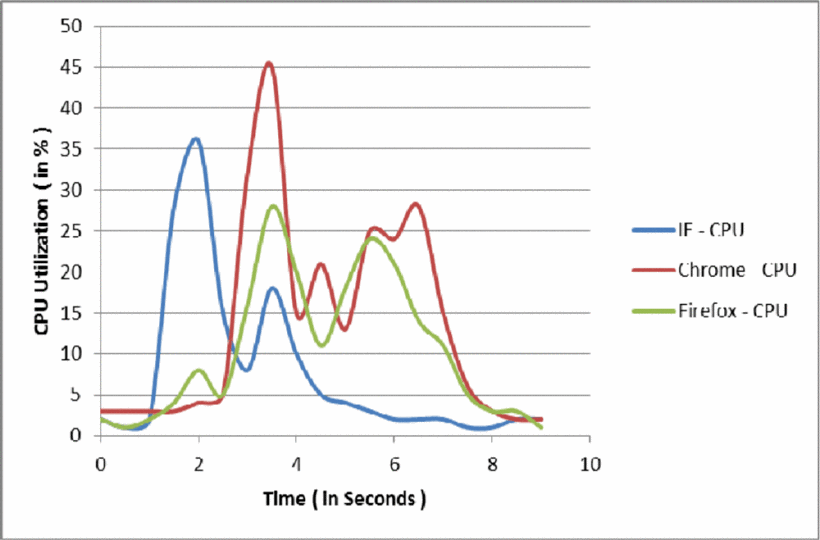
\includegraphics[scale=0.25]{figures/einleitung/browser_comparisson.png}
	\caption{Browser CPU utilization comparison\cite{6724273}}
	\label{browser_comp}
\end{figure}
\\
There are already some alternative libraries on the internet to recreate this method, but most of them are written in other programming languages. Adding them to a C++ Project would rise the complexity of the source code.\\
Some people would think "Well C++ is a new and modern language. There must be something similar out there". This statement is true and because of its young age there are a limited number of officially tested methods. You could also take a look at the headers implemented in the \href{https://en.cppreference.com/w/cpp/header}{C++ standard library} \cite{CppRef} to familiarize yourself with common algorithms and data structures.

\section{Obective}
The purpose of this thesis is the development, implementation and testing of a Library for C++ applications that creates an artificial workload and delivers system independent statistics based on multi-threading. This will allow developers to implement their own stress tests and run simulations with different workloads, process priorities and scheduling, which can be used in different manners to achieve real-time applications. These could be later automatized by using programs like \href{https://www.jenkins.io/}{Jenkins}\cite{Jenkins} or \href{https://about.gitlab.com/}{Gitlab}\cite{GitLab}.

\section{Implementation}
The library has two main components. The first one is the workload, which can vary depending of the user's input. This will create a system specific amount of threads and make them run a simulation function. The number of threads will stay constant and the time for running the workload task will be set accordingly for each input.\\
The second components is the system. This comes with functions, which can easily change a thread's priority, a system's scheduling policy and deliver statistics of the user's computer.\\
Basic operations are implemented to work on most operating systems, but there are some exceptions because of the differences between OS implementations, which makes them independent from one another.
\section{Advantages and Disadvantages}
\subsection{Pros}
\begin{enumerate}
	\item No additional expenses for third party software or subscriptions
	\item Can be directly added to the source code, which makes testing easy
	\item No external influence from the browser(ads) or internet connection, allowing efficient testing even offline
	\item Allows the creation of tests based on user experience 
	\item Companies don't have to give their data 
\end{enumerate}

\subsection{Cons}
\begin{enumerate}
	\item Tests don't come already prepared
	\item Developers have add the source code to their build system or add the build files to their own if they already use CMake
\end{enumerate}
\subsection{Summary}
With this library a company can save money, improve their product based on user feedback and create an internet independent test system for very minimal effort.